\documentclass[11pt]{article}
\usepackage[letterpaper, margin=0.5in, includeheadfoot]{geometry}
% \usepackage[myheadings]{fullpage}
\usepackage{fancyhdr}
\usepackage{lastpage}
\usepackage{graphicx, wrapfig, subcaption, setspace, booktabs}
\usepackage[T1]{fontenc}
\usepackage[font=small, labelfont=bf]{caption}
\usepackage{fourier}
\usepackage[protrusion=true, expansion=true]{microtype}
\usepackage[english]{babel}
\usepackage[final]{hyperref}
\usepackage{sectsty}
\usepackage{cite}
\usepackage{url, lipsum}
\usepackage{float}
\usepackage{amsmath}
%\usepackage{mathpazo}
\usepackage{mathtools}
\usepackage{xcolor}
\newcommand{\HRule}[1]{\rule{\linewidth}{#1}}
\onehalfspacing
\setcounter{tocdepth}{5}
\setcounter{secnumdepth}{5}
\usepackage{hanging}
\usepackage{matlab-prettifier}
\usepackage{pdfpages}
%-------------------------------------------------------------------------
% HEADER & FOOTER
%-------------------------------------------------------------------------
\pagestyle{fancy}
\fancyhf{}
\setlength\headheight{15pt}
\fancyhead[L]{Jack Hickisch}
\fancyhead[R]{MATH550 | HOMEWORK \#0}
\fancyfoot[R]{Page \thepage\ of \pageref{LastPage}}
%-------------------------------------------------------------------------
% TITLE PAGE
%-------------------------------------------------------------------------
\begin{document}
\title{ \normalsize \textsc{}
\\ [0.0cm]
\HRule{1pt} \\
\Large \textbf{\uppercase{MATH550 | HOMEWORK \#0}} \\
\HRule{1pt} \\
\vspace*{0.25\baselineskip}
\date{September 17, 2026}
\author{Jack Hickisch}}

\maketitle

\begin{abstract}
\noindent
This report assumes familiarity with the assignment as provided by Dr. Sprinkle. Most problems only include a plot and brief description as requested.
\end{abstract}

\pagebreak

\section{Problem 1: Finite Differences \& Problem 2: Second-order Derivatives}

\begin{figure}[H]
    \centering
    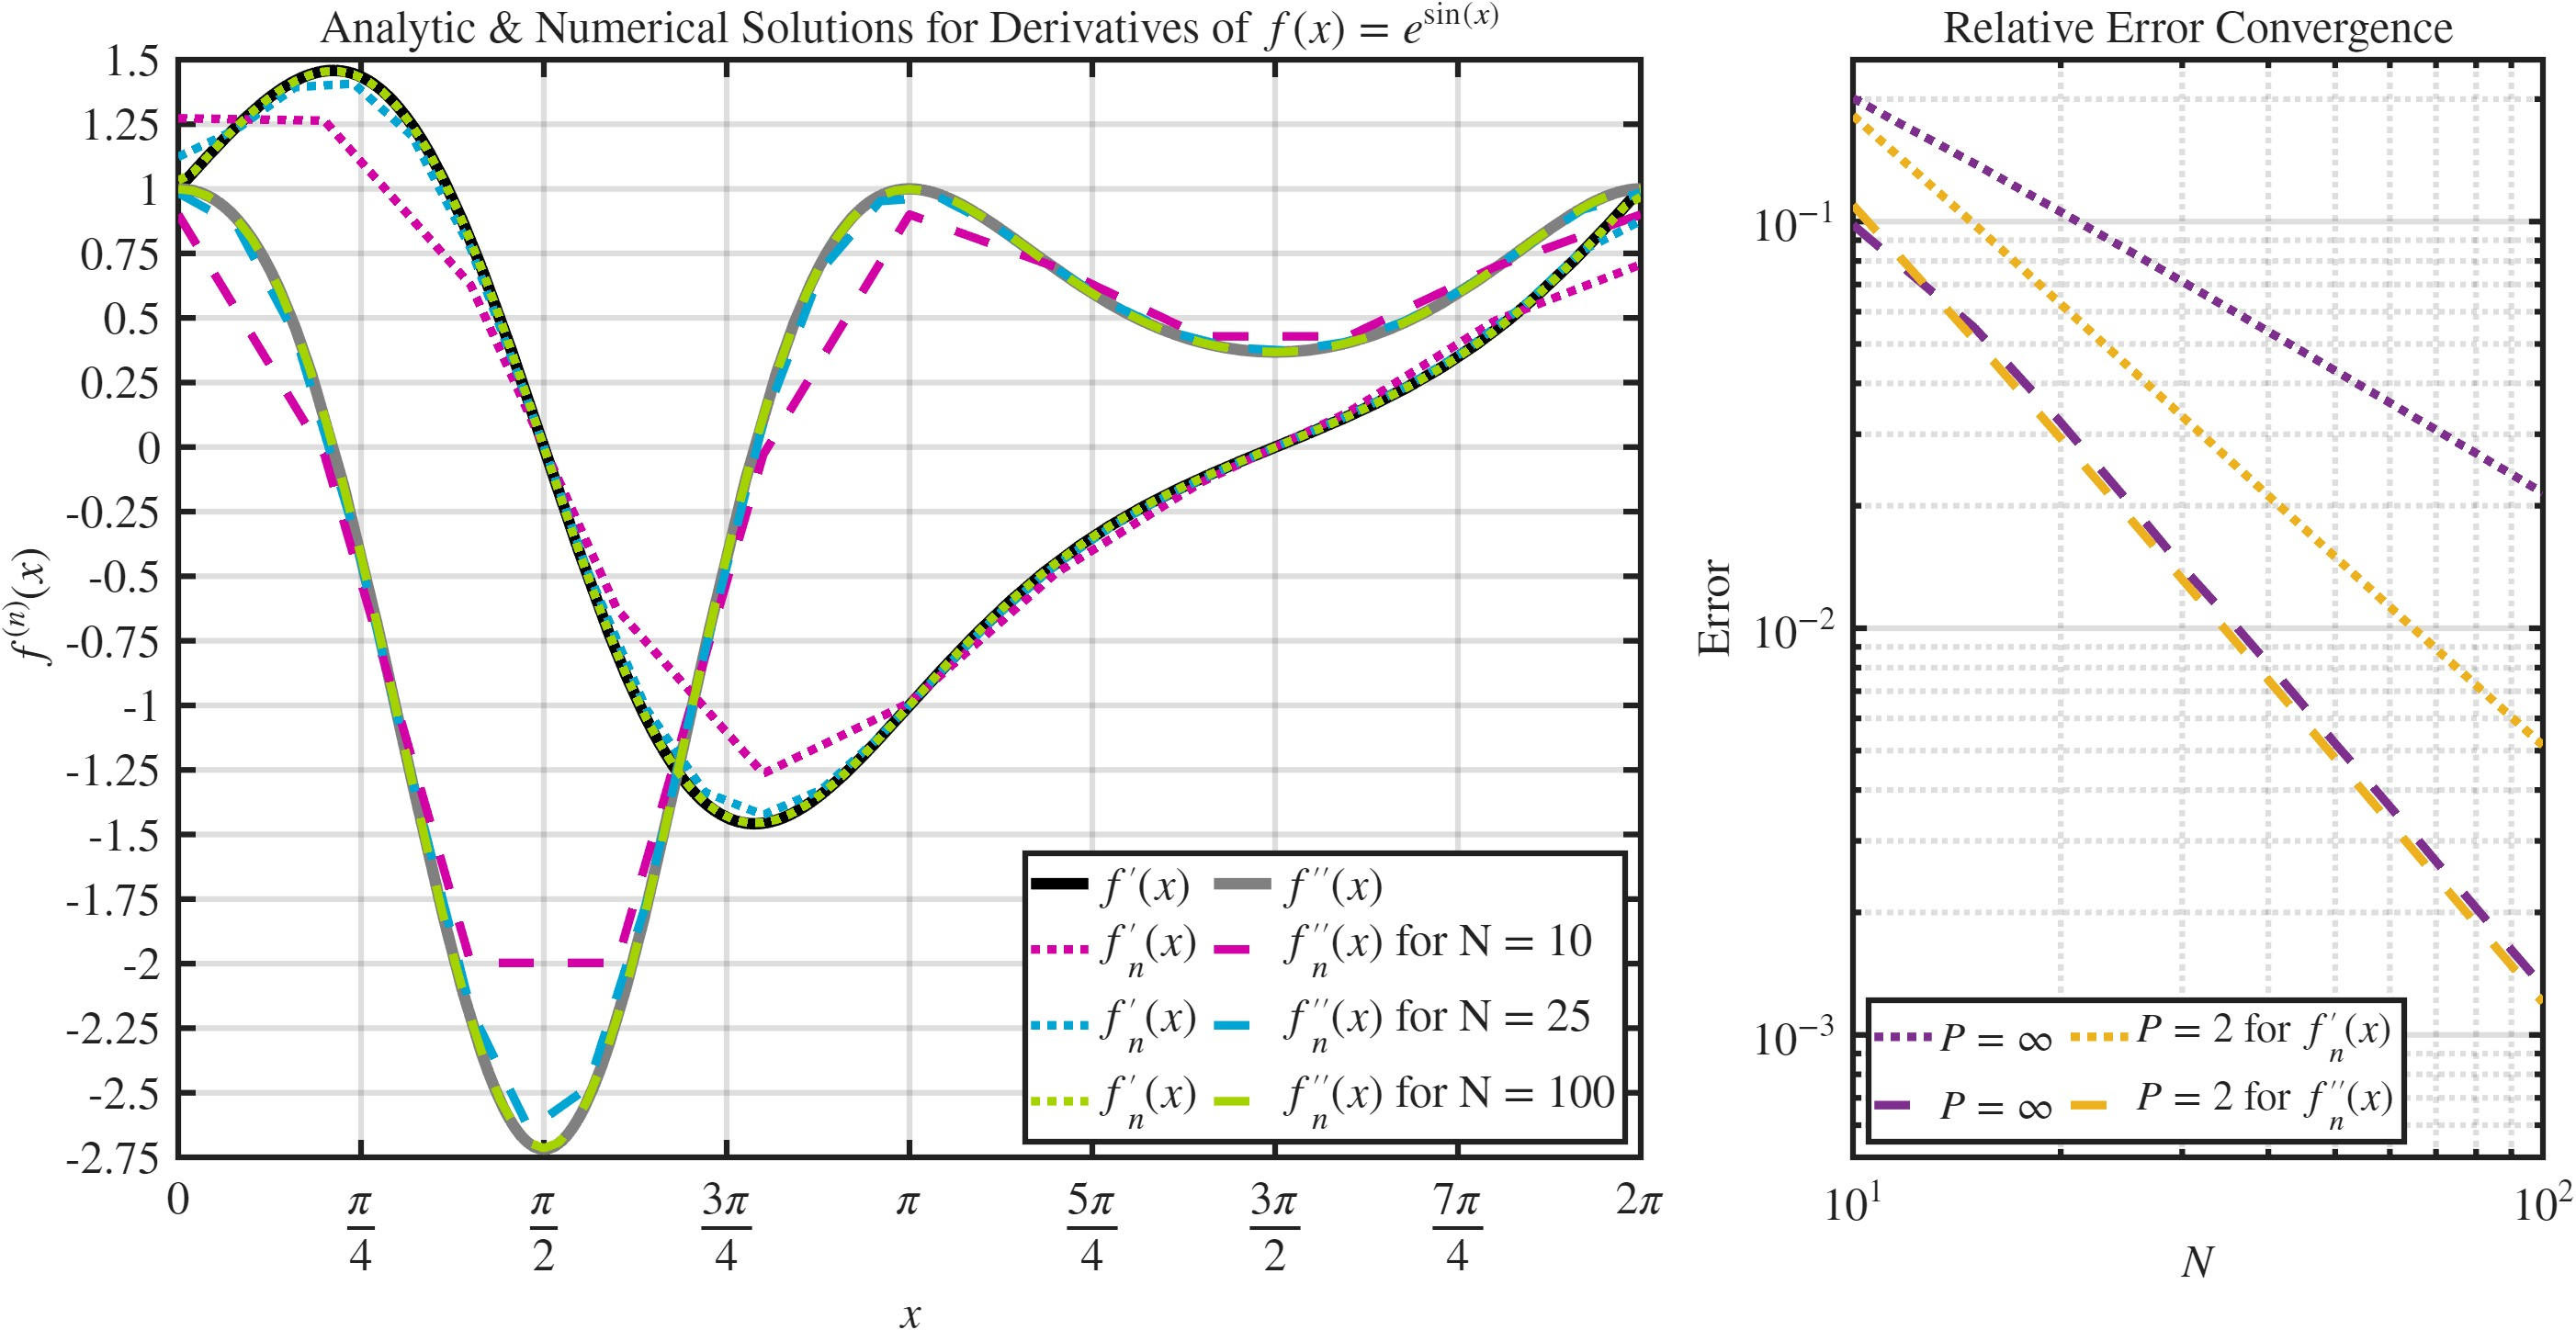
\includegraphics[width=1\linewidth]{HW0_1and2.jpg}
    \caption{Function and Error Plot}
    \label{fig:1}
\end{figure}

\noindent The $P=2$ error plot slope is $-3/2$ for the first derivative because there is a mix of first order (used on the boundaries) and second order (used for the non-boundaries) accurate methods. 

\section{Problem 3: ODE}

\begin{figure}[H]
    \centering
    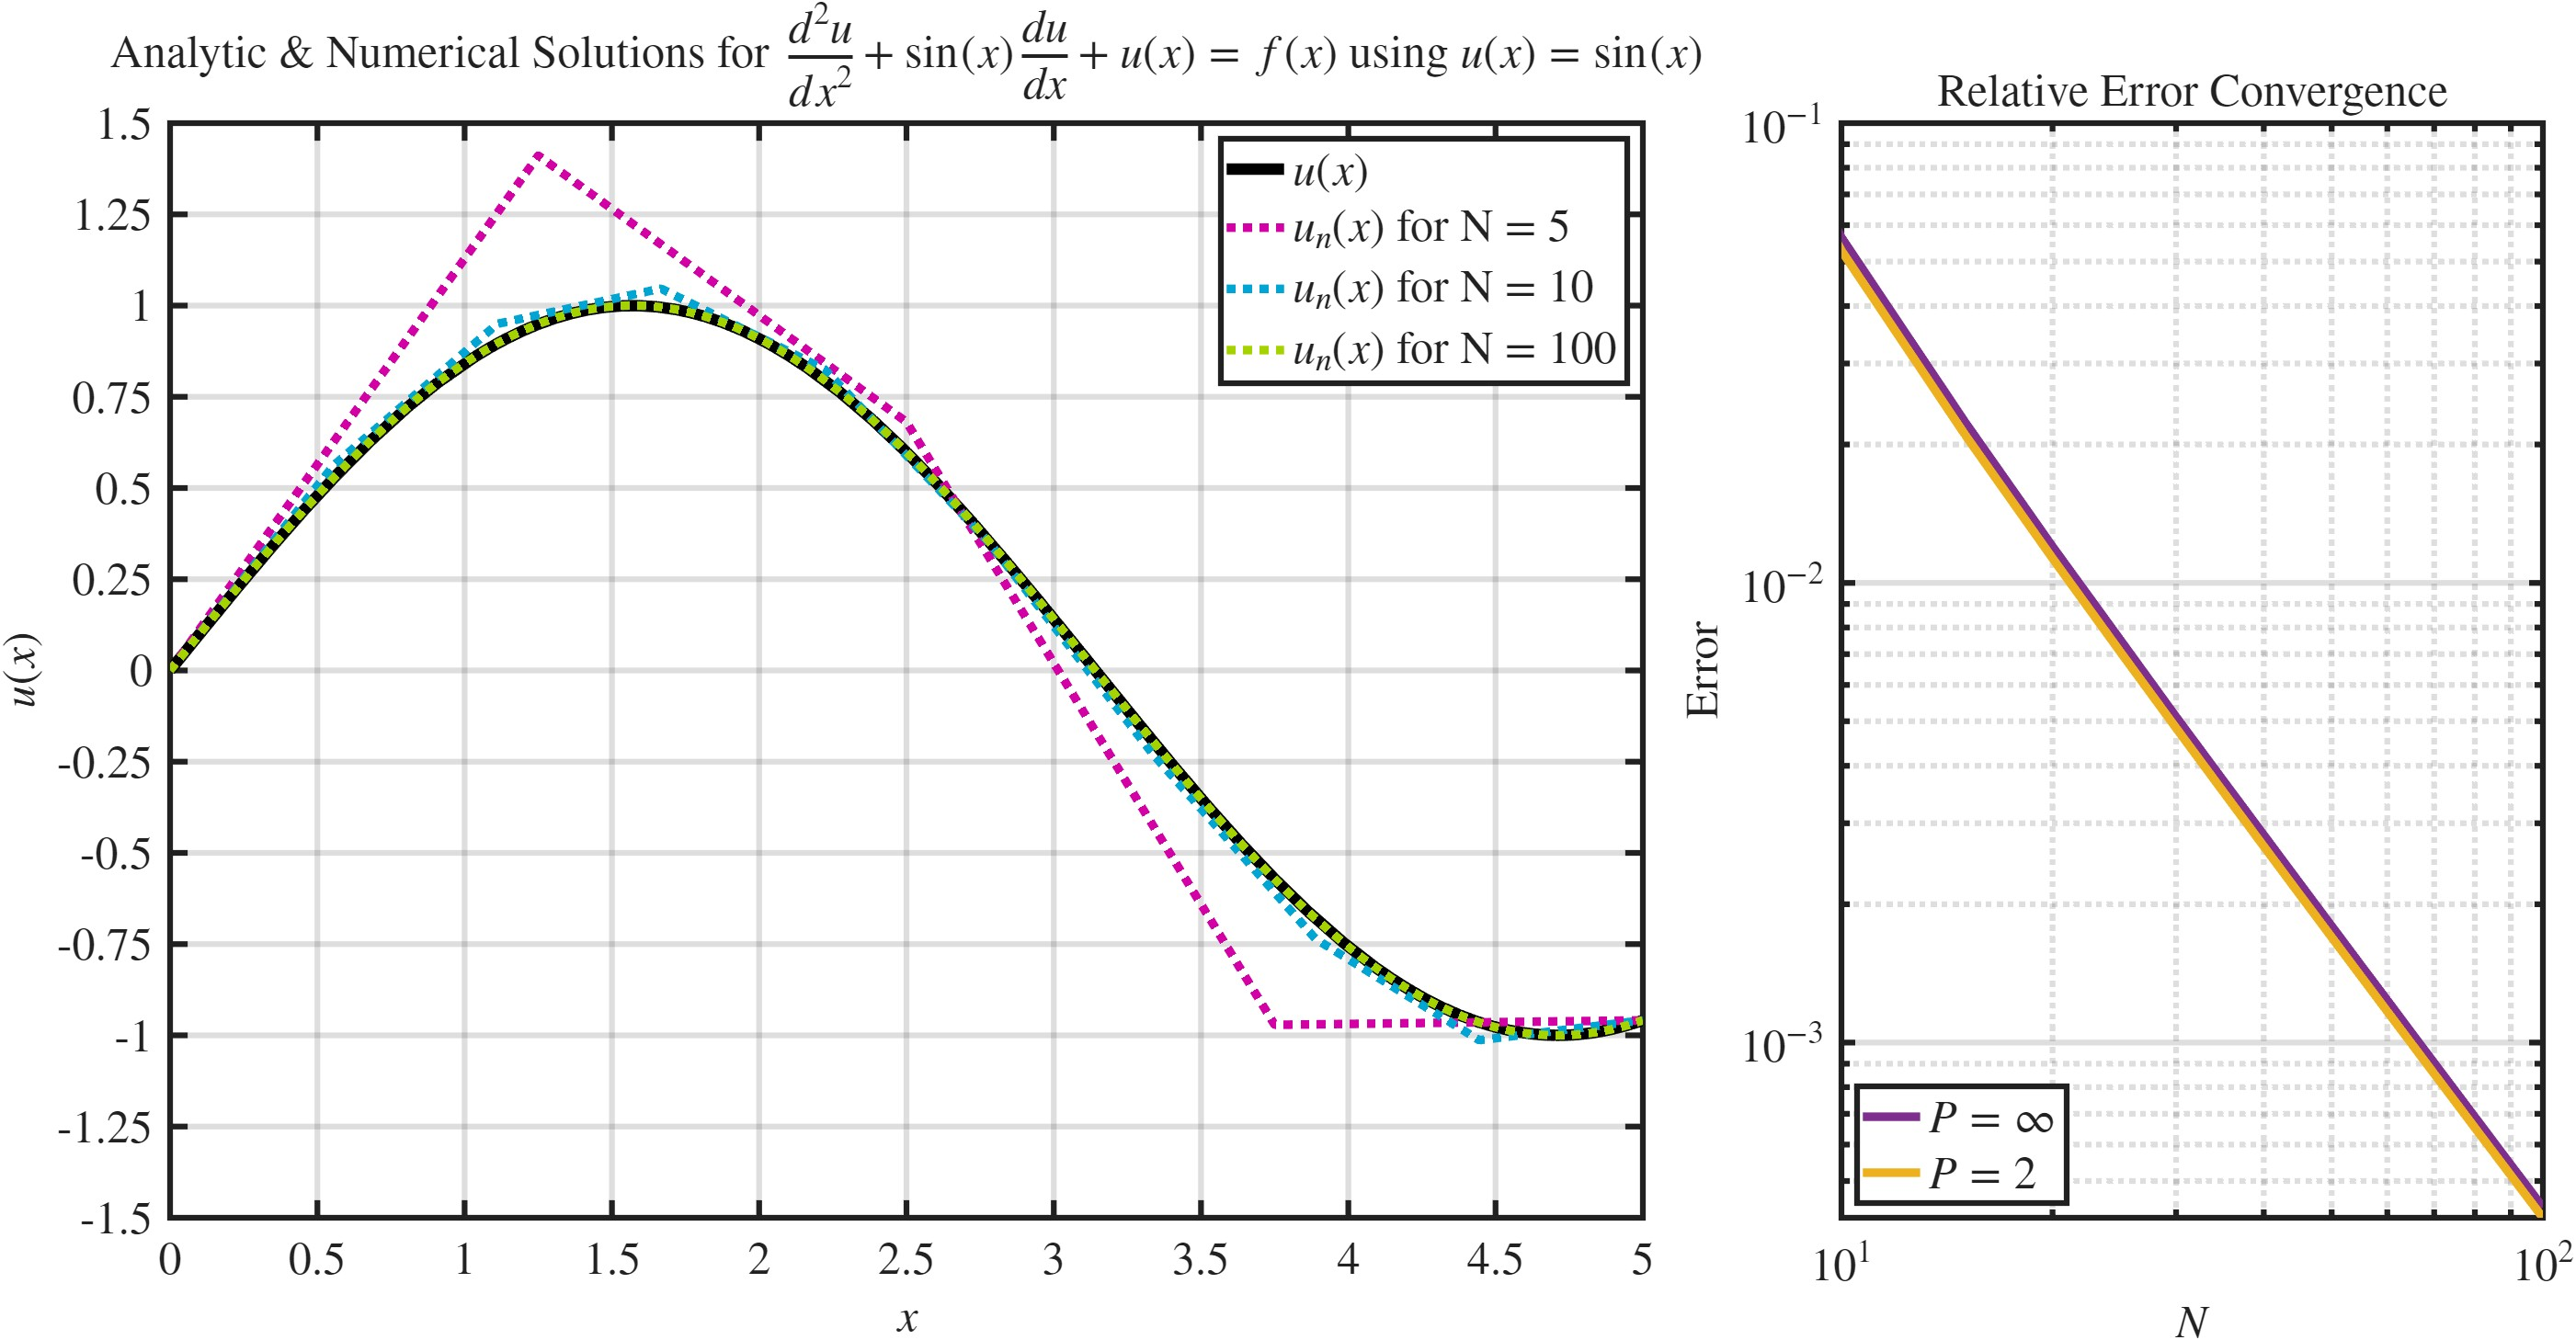
\includegraphics[width=1\linewidth]{HW0_3.jpg}
    \caption{Function and Error Plot}
    \label{fig:2}
\end{figure}

\noindent For the solution $u(x)=\sin(x)$ to be valid, the forcing function must be set to $f(x)=\sin(x)\cos(x)$. The code sets the boundaries as follows: $u(0)=\sin(0)=0$ and $u(5)=\sin(5)\approx-0.95892$. The slope of the convergence plot is $-2$ because second-order finite difference methods are employed over the entire domain.

\section{Problem 4: Poisson Equation}

\begin{figure}[H]
    \centering
    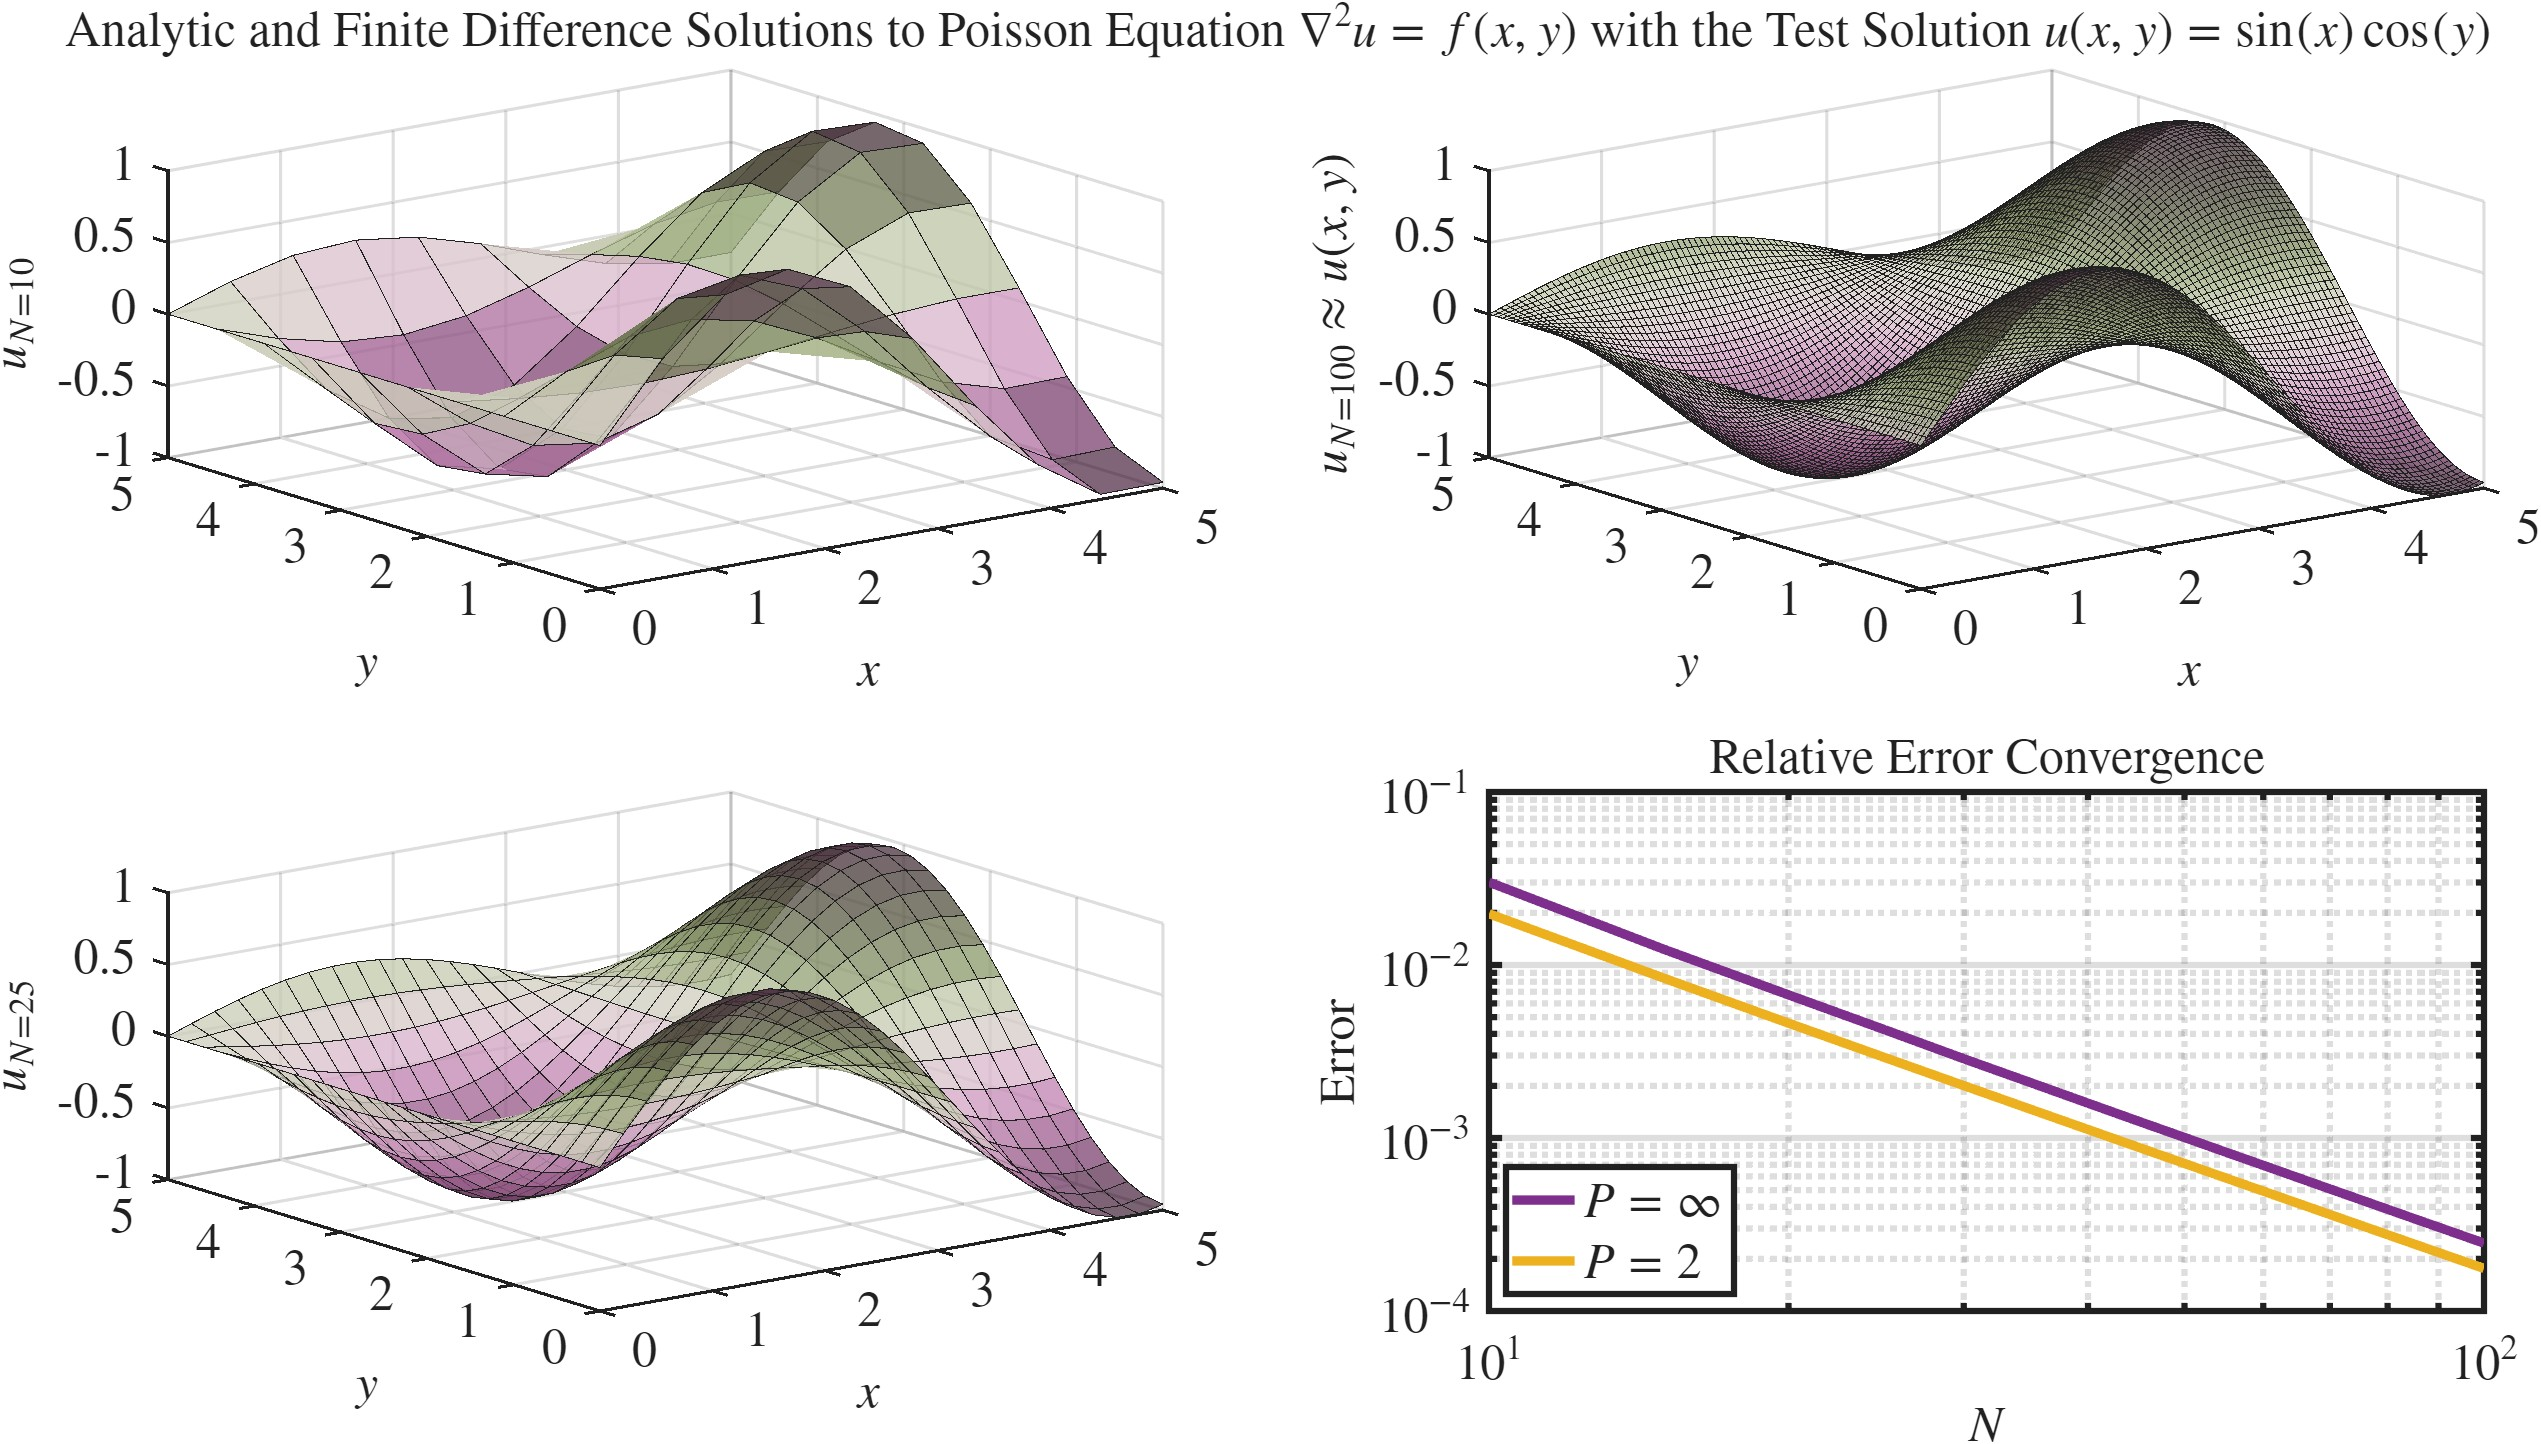
\includegraphics[width=1\linewidth]{HW0_4.jpg}
    \caption{Function and Error Plot}
    \label{fig:3}
\end{figure}

\subsection{Part 1}

\noindent For the solution $u(x)=\sin(x)\cos(y)$ to be valid, the forcing function must be set to $f(x)=-2\sin(x)\cos(y)$. To determine the boundary conditions, $u(x)=\sin(x)\cos(y)$ is evaluated for each edge of the domain. The slope of the convergence plot is $-2$ because second-order finite difference methods are employed over the entire domain.

\subsection{Part 2}

If Neumann (derivative) boundary conditions were to be employed the PDE would be indeterminate and have infinity many solutions. This is because there would be no way to set the "constant of integration" for the function. To fix this, in addition to Neumann conditions being applied, any singular point on the grid could be set to any value which would "pin" the solution to the PDE in place. Alternatively, an equation could be added that forces the sum of all grid values to be zero. This would effectively "center" the solution to the PDE around $0$.



\section{Commented Code}

\noindent Commented MATLAB Code is provided below.

\subsection{Problems 1 \& 2}
\lstinputlisting[style=Matlab-editor]{MATH550_HW_0_Problem1.m} %Code
\subsection{Problem 3}
\lstinputlisting[style=Matlab-editor]{MATH550_HW_0_Problem3.m} %Code
\subsection{Problem 4}
\lstinputlisting[style=Matlab-editor]{MATH550_HW_0_Problem4.m} %Code



\section{References}

\noindent The original assignment description(s) are provided below along with scratch work.

\includepdf[pages=-]{Scratch Work.pdf} %Scratch Work

\includepdf[pages=-]{Assignment.pdf} %Assignment

\end{document}
